\chapter{Teoria das Redes de Petri Hierárquicas de Sinais}
\label{ch:shpn}

Este capítulo apresenta a definição matemática formal das Redes de Petri
Hierárquicas de Sinais (SHPN), estendendo a 5-tupla canônica $(P, T, F, W, M_0)$
a uma 13-tupla que incorpora organização hierárquica de sinais, realismo
biológico e fundamentação termodinâmica dos limiares de habilitação.
O qualificativo \emph{hierárquicas} refere-se à estratificação dos
\textbf{sinais} pela função de camada $\lambda: \Psi \to \mathbb{N}$, não à
composição hierárquica de sub-redes no sentido de Jensen~\cite{Jensen1997CPN} ---
a topologia da rede permanece plana. A Seção~\ref{sec:definicao-13tupla} especifica o formalismo completo.
A Seção~\ref{sec:componentes-sinal} detalha os componentes de sinal. A
Seção~\ref{sec:semantica-operacional} formaliza a semântica operacional. A
Seção~\ref{sec:propriedades-teoricas} estabelece as garantias teóricas.

\section{A Definição Formal da 13-Tupla}
\label{sec:definicao-13tupla}

\begin{definition}[Rede de Petri Hierárquica de Sinais]
\label{def:shpn}
Uma Rede de Petri Hierárquica de Sinais é uma 13-tupla:
\[
N = (P,\; T,\; F,\; W,\; M_0,\; \Phi,\; C,\; F_t,\; \Psi,\; F_s,\; W_s,\; \lambda,\; \Gamma)
\]
em que:
\begin{itemize}
  \item $P$ é um conjunto finito de lugares (espécies moleculares, estados
        celulares);
  \item $T$ é um conjunto finito de transições (reações, eventos regulatórios),
        com $P \cap T = \emptyset$;
  \item $F \subseteq (P \times T) \cup (T \times P)$ são os arcos orientados
        (arcos normais, estequiométricos);
  \item $W: F \to \mathbb{R}^+$ são os pesos dos arcos normais, generalizados
        a \textbf{expressões reais sobre a marcação}, $W \in \mathbb{E}(M)$
        (a álgebra das expressões aritméticas sobre $M$, constantes e funções
        elementares); o caso clássico $W \equiv k$ é recuperado tomando
        constantes;
  \item $M_0: P \to \mathbb{R}_{\geq 0}$ é a marcação inicial;
  \item $\Phi: T \to \{\text{contínua, estocástica, imediata, temporizada,
        burst}\}$ é a função de tipo de transição; a lei cinética
        $r_t \in \mathbb{E}(M, \Gamma, t)$ associada a $\Phi(t)$ é, em
        geral, uma expressão real sobre a marcação, sobre a tupla
        termodinâmica $\Gamma$ e sobre o tempo;
  \item $C: P \to \mathcal{C}$ é a função de atribuição de compartimento
        (e.g.\ citoplasma, núcleo, mitocôndria); determina a conversão
        token$\to$concentração via $V_{C(p)}$ e a fronteira termodinâmica
        de cada espécie. A identidade química das espécies (fórmulas
        moleculares, SMILES, InChI) é tratada como metadado descritivo
        externo à tupla formal — o lugar é identificado pelo seu nome/ID;
        $C$ define apenas o ambiente volumétrico para conversão de unidades;
  \item $F_t \subseteq P \times T$ são os arcos de teste (clássicos, na
        linhagem de Koch~\cite{Koch2011} e Heiner~\cite{Heiner2008}). O
        conjunto $F_t$ admite \emph{refinamento de tipo de arco} interno em
        duas variantes — \textbf{teste} (catálise não consuntiva, habilita
        sse $M(p) > \tau_t((p,t))$) e \textbf{inibidor} (David \&
        Alla~\cite{David1992}, Heiner~\cite{Heiner2008}; desabilita sse
        $M(p) \geq \theta_i((p,t))$). Ambos os limiares $\tau_t, \theta_i
        \in \mathbb{E}(M)$ são expressões reais sobre a marcação; o caso
        clássico de limiar inteiro constante é recuperado por especialização.
        Esta diferenciação é \textbf{textual}, à maneira da própria
        diferenciação clássica entre arcos de entrada e arcos de saída em
        $F$, e \emph{não} introduz novo elemento na tupla;
  \item $\Psi \subseteq P$ é o conjunto de \textbf{lugares de sinal} --- as
        espécies que intermediam controle regulatório além de transferência de massa;
  \item $F_s \subseteq (\Psi \times T) \cup (T \times \Psi)$ são os
        \textbf{arcos de fluxo de sinal} (transformação de informação com
        consumo);
  \item $W_s: F_s \to \mathbb{R}^+$ são os pesos dos arcos de fluxo de sinal,
        igualmente em $\mathbb{E}(M)$;
  \item $\lambda: \Psi \to \mathbb{N}_0$ é a \textbf{função de camada
        hierárquica} (metabolismo $= 0$, sinalização $= 1$, transcrição $= 2$,
        \ldots);
  \item $\Gamma = (K, n, \varepsilon)$ é a \textbf{tupla de restrição
        termodinâmica}, em que $K: F_s \to \mathbb{R}^+$ são as constantes
        de Michaelis por arco de sinal (mensuráveis via cinética enzimática),
        $n: F_s \to \mathbb{N}^+$ são os coeficientes de Hill por arco
        (mensuráveis via curvas dose-resposta), e
        $\varepsilon \in (0,1)$ é o limiar universal de supressão de taxa
        (constante do formalismo, e.g.\ $\varepsilon = 0{,}05$ para 5\% de
        atividade residual) --- ver Seção~\ref{subsec:limiares}.
\end{itemize}
\end{definition}

A definição estende a 5-tupla clássica com três componentes biológicos
($\Phi, C, F_t$) e cinco componentes de hierarquia de sinais ($\Psi, F_s, W_s,
\lambda, \Gamma$). Atribuindo $\Psi = \emptyset$ obtém-se uma Rede de Petri
Biológica clássica; atribuindo adicionalmente $F_t = \emptyset$, $C = $ função
constante e $\Phi = $ tipo único recupera-se exatamente a 5-tupla canônica.

\begin{remark}[Refinamento textual de componentes clássicos]
\label{rem:refinamento-textual}
A estratégia segue a própria convenção clássica das Redes de Petri: o
conjunto $F$ não é fatorado na tupla em \emph{arcos de entrada} e
\emph{arcos de saída}, embora a definição operacional os trate de modo
distinto; a diferenciação ocorre no texto. Pelo mesmo princípio, a
\textbf{redefinição} de componentes que já figuram no formalismo clássico
— a generalização de $W$, $W_s$ e das leis cinéticas associadas a $\Phi$
de constantes para expressões em $\mathbb{E}(M)$, e a partilha de $F_t$
entre as variantes \emph{teste} e \emph{inibidor} — \emph{não} produz
novos elementos da tupla. A 13-tupla é estendida apenas com conceitos
estruturalmente novos (lugares de sinal $\Psi$, arcos de fluxo de sinal
$F_s$, função de camada $\lambda$, parâmetro termodinâmico $\Gamma$).
\end{remark}

A decisão de substituir o parâmetro estático $\theta$ pela tupla
$\Gamma = (K, n, \varepsilon)$ elimina uma circularidade conceitual: em
formulações anteriores, $\theta$ recebia um valor emergente medido
experimentalmente (e.g.\ $\theta_{\sigma H} \approx 1{,}60\,\mu$M de $\sigma^H$
na esporulação de \textit{B.~subtilis}, separatriz de comprometimento
identificada por \textcite{Fujita2005}) e o reclassificava
como constante estática.  No presente formalismo, o limiar efetivo por arco
$\theta_{\mathrm{eff}}$ é \emph{derivado analiticamente} a partir de
constantes cinéticas diretamente mensuráveis; contudo, o \textbf{ponto de
comprometimento sistêmico} --- a concentração e o instante temporal em que a
rede acoplada se compromete irreversivelmente --- \emph{emerge} da simulação
dinâmica, pois depende da interação entre regeneração de ATP, consumo pela
cascata e inibição por produto, não sendo computável pela fórmula isoladamente.
Essa separação entre derivação analítica por arco e emergência sistêmica torna
a predição genuinamente \emph{orientada pela topologia}.

\begin{remark}[Generalidade de $\Gamma$ além de sinais energéticos]
\label{rem:gamma-generalidade}
A tupla $\Gamma = (K, n, \varepsilon)$ é denominada ``termodinâmica'' porque
a demonstração empírica desta tese emprega o $\sigma^H$ --- o portador de
comprometimento cuja constante cinética $K$ na função de taxa de $T_{\text{septação}}$
relação-se diretamente com a afinidade enzimática da cascata sigma. O ATP
no Capítulo~\ref{ch:validacao-bacillus} participa como substrato metabólico
(arcos normais $F$) --- uma instância particular escolhida pela disponibilidade de
dados cinéticos publicados --- e não como o sinal de comprometimento.

As propriedades formais demonstradas neste capítulo --- os Teoremas de Aciclicidade
(Seção~\ref{subsec:aciclicidade}), Garantia de Preempção
(Seção~\ref{subsec:corretude-preempcao}), Formação de Fronteiras de Bacia
(Seção~\ref{subsec:fronteiras-bacia}) e Independência Fraca
(Seção~\ref{subsec:independencia-fraca}) --- é independente da natureza
física do sinal: as provas requerem apenas que $p_s \in \Psi$, que $(K, n)$
sejam reais positivos e que $\varepsilon \in (0,1)$, sem qualquer hipótese
sobre o sinal ser energético, transcricional ou de outra natureza.

Em consequência, o formalismo aplica-se a qualquer lugar que o modelador
designe como sinal: fatores de transcrição (e.g.\ Spo0A${\sim}$P, com $K$
derivado da afinidade de ligação ao DNA), morfógenos (e.g.\ Bicóide em
\textit{Drosophila}, com $n \approx 5$ para ativação cooperativa de
\textit{hunchback}), sinais de \textit{quorum sensing} (e.g.\ AHL, com $K$ do
receptor LuxR), segundos mensageiros (e.g.\ cAMP, com $K_{0{,}5}$
alostérico) e hormônios (e.g.\ insulina, com $K_d$ do receptor)~\cite{Simao2026QuorumSensing}.  O ATP
no Capítulo~\ref{ch:validacao-bacillus} é uma instância particular ---
escolhida pela disponibilidade de medida experimental de limiar --- e não uma
restrição do formalismo.
\end{remark}

\section{Componentes de Sinal}
\label{sec:componentes-sinal}

\subsection{Lugares de Sinal}
\label{subsec:lugares-sinal}

Os \textbf{lugares de sinal} $\Psi \subseteq P$ particionam as espécies
moleculares entre aquelas que participam de transferência de massa e aquelas que
intermediam informação regulatória. Um lugar $p \in \Psi$ pode ter
simultaneamente arcos normais (para a cinética enzimática) e arcos de fluxo de
sinal (para o controle regulatório), formalizando a dualidade metabolito-sinal
descrita na introdução.

O ATP exemplifica essa dualidade: como substrato da glicólise participa por
arcos normais (consumo/produção estequeométrico); como sinal na decisão de
esporulação participa por arcos de fluxo de sinal (consumo regulatório com
limiar $\theta_{\mathrm{eff}}$). O mesmo lugar pertence a $\Psi$ e opera em ambas as semânticas
simultaneamente.

\begin{principle}[Separação Vertical-Horizontal]
\label{princ:separacao}
Os arcos normais $F$ modelam transferência de massa no plano horizontal
(metabolismo, estequiometria). Os arcos de fluxo de sinal $F_s$ modelam
transferência de informação no eixo vertical (hierarquia regulatória). Essa
separação torna o formalismo composicionalmente tratável.
\end{principle}

\subsection{Arcos de Fluxo de Sinal}
\label{subsec:arcos-sinal}

Os \textbf{arcos de fluxo de sinal} $F_s \subseteq (\Psi \times T) \cup
(T \times \Psi)$ implementam transformação de informação com consumo
estequiométrico. O peso $W_s((p_s, t))$ especifica a quantidade de token de
sinal consumida quando $t$ dispara a partir de $p_s \in \Psi$.

A distinção fundamental entre os três tipos de arcos é: os arcos normais $F$
modelam o que é transferido (massa no nível metabólico); os arcos de fluxo de
sinal $F_s$ modelam como a informação se propaga (estado de concentração
transmitido aos níveis regulatórios); os arcos de teste $F_t$ observam sem
consumir (catálise enzimática genuína). As três semânticas coexistem dentro do
mesmo formalismo.

\begin{remark}[Arquitetura Dual: Grafo Executório e Grafo de Controle]
\label{rem:dual-graph}
A estrutura das SHPN pode ser interpretada como a superposição de dois grafos
funcionalmente distintos. O \textbf{grafo executório} é constituído pelos
lugares metabólicos $P \setminus \Psi$, pelas transições e pelos arcos normais
$F$: é a \emph{planta} no sentido da teoria de controle --- executa
transformações bioquímicas, conserva massa e aplica estequiometria, sem
qualquer consciência de propósito ou estado global. O \textbf{grafo de controle}
é constituído pelos lugares de sinal $\Psi$, pelos arcos de fluxo de sinal $F_s$
e pela função de camada $\lambda$: é o \emph{controlador} --- mantém estado
sobre o estado do sistema, avalia limiares e determina quais transições do grafo
executório estão habilitadas a disparar.

Os arcos de fluxo de sinal $F_s$ são os \textbf{canais de observação} que
conectam os dois grafos. Um arco $(p_s, t) \in F_s$, com $p_s \in \Psi$,
funciona como um fio sensor: lê a marcação atual de $p_s$ no grafo executório e
projeta essa informação para dentro do grafo de controle, onde é avaliada em
relação ao limiar $\theta_{\mathrm{eff}}(p_s,t)$. A semântica consuntiva dos arcos de sinal é
essencial: o token de sinal é \emph{consumido} na avaliação, o que significa que
a informação é utilizada para produzir a decisão de controle e não pode ser
reutilizada sem nova produção --- formalizando o comportamento de sensores
moleculares reais que são ativados e depois retornam ao estado basal.

O ciclo de realimentação resultante é:
\[
\underbrace{M(p_s)}_{\text{grafo executório}}
\xrightarrow{\ F_s \text{ (observação)}\ }
\underbrace{\text{avaliação de } \theta(t)}_{\text{grafo de controle}}
\xrightarrow{\ \text{habilita/inibe}\ }
\underbrace{\text{disparo de } t}_{\text{grafo executório}}
\]

A potência desta arquitetura reside no fato de que a mesma molécula --- por
exemplo, o ATP --- pode participar \emph{simultaneamente} dos dois grafos: como
substrato no grafo executório (arcos normais, consumo estequiométrico na
glicólise) e como sinal no grafo de controle (arco de fluxo de sinal, detecção
de limiar na decisão de esporulação). Não é necessário duplicar o lugar nem
escolher uma semântica em detrimento da outra.
\end{remark}

\subsection{Duas Decisões Ortogonais do Modelador}
\label{subsec:decisoes-modelador}

A construção de uma SHPN exige do modelador \emph{duas decisões
independentes}, cuja combinação determina a capacidade preditiva do modelo.

A primeira é a \textbf{designação de atuação}: decidir, para cada lugar
$p \in P$, se $p \in \Psi$. Trata-se de uma anotação semântica --- o lugar
carrega informação regulatória além de, possivelmente, massa --- e não de uma
propriedade topológica. O mesmo metabólito pode atuar como sinal em um modelo
e como mero substrato em outro, conforme a pergunta biológica em foco.

A segunda é o \textbf{tipo do arco de leitura}: decidir, para cada transição
que sonda $p \in \Psi$, se a leitura é \emph{não-consuntiva} ($F_t$) ou
\emph{consuntiva} ($F_s$). Apenas a leitura consuntiva depleta o sinal e,
portanto, cria fronteira de bacia.

A Tabela~\ref{tab:decisoes-modelador} resume as combinações relevantes
e sua interpretação biológica.

\begin{table}[htbp]
\centering
\caption{Combinações entre designação $\Psi$ e tipo de arco incidente
sobre um lugar $p \in P$. A capacidade de predizer limiares de decisão
depende exclusivamente da quarta linha (sinal lido por $F_s$).}
\label{tab:decisoes-modelador}
\renewcommand{\arraystretch}{1.25}
\small
\begin{tabularx}{\textwidth}{@{}c c l X@{}}
\toprule
\textbf{$p \in \Psi$?} & \textbf{Arco} & \textbf{Semântica de leitura} & \textbf{Exemplo biológico} \\
\midrule
não & $F$   & estequiometria pura              & glicose como substrato \\
não & $F_t$ & catálise não-consuntiva          & enzima sobre substrato \\
sim & $F$   & participação metabólica do sinal & ATP $\to$ ADP na glicólise \\
sim & $F_t$ & sondagem regulatória sem consumo & KinA detecta ATP sem depletá-lo \\
sim & $F_s$ & \textbf{consuntiva $\Rightarrow$ fronteira de bacia} & GTP\_pool $\to$ $T_{\text{septação}}$ na esporulação \\
\bottomrule
\end{tabularx}
\end{table}

A ortogonalidade entre as duas decisões de modelagem é essencial:
declarar $p \in \Psi$ \emph{não} obriga que todas as transições
leitoras de $p$ usem $F_s$. Catálise enzimática genuína sobre um lugar de sinal
permanece corretamente representada por $F_t$ --- por exemplo, uma
enzima reguladora que se liga a Spo0A${\sim}$P sem o consumir age como
sensor não-consuntivo, ainda que Spo0A${\sim}$P seja sinal regulatório
em outras transições da mesma rede.

\begin{remark}[Decisão silenciosa de modelagem]
\label{rem:decisao-silenciosa}
A escolha incorreta entre $F_t$ e $F_s$ \emph{não} produz erro de
simulação: o modelo carrega, executa e gera trajetórias numericamente
plausíveis. O que se perde é a \emph{capacidade preditiva}: substituir
$F_s$ por $F_t$ sobre o sinal de comprometimento elimina o consumo,
suprime a fronteira de bacia e torna formalmente inexprimível a
pergunta ``a partir de qual concentração a célula se compromete?''.
A demonstração formal dessa perda figura no
Capítulo~\ref{ch:validacao-bacillus},
Seção~\ref{sec:comparacao-classicas}, contrastando o modelo SHPN com
sua versão de arcos de teste. A designação $\Psi$ e a atribuição de
$F_t$ versus $F_s$ constituem, portanto, decisões críticas de
modelagem que devem preceder qualquer escolha de parâmetros
cinéticos.
\end{remark}

\subsection{Função de Camada Hierárquica}
\label{subsec:funcao-camada}

A \textbf{função de camada hierárquica} $\lambda: \Psi \to \mathbb{N}_0$ atribui
a cada lugar de sinal um nível organizacional com regras de precedência. A
atribuição segue a ordenação topológica do grafo de fluxo de sinal dirigido:
lugares de sinal fonte (sem arcos entrantes em $F_s$) recebem camada~0;
lugares dependentes recebem camada $\max\{\lambda(q)\} + 1$ sobre todos os
sinais antecessores $q$.

Na esporulação de \textit{B.~subtilis}: KinA$_{\text{kinase}}$ pertence à
camada~0 (sensor de privação nutricional), Spo0A${\sim}$P à camada~1
(integração da fosforretransmissão), $\sigma^H$ à camada~2 (portão de
comprometimento), e $\sigma^F$/$\sigma^E$ à camada~3 (execução). A
preempção hierárquica resulta naturalmente: quando $\sigma^H$ (camada~2) fica
abaixo da separatriz $\theta_{\sigma H} \approx 1{,}60\,\mu$M, todas as transições
que dependem dos sinais da camada~3 são desabilitadas.

\subsection{Limiares de Habilitação e Fundamentação Termodinâmica}
\label{subsec:limiares}

A tupla termodinâmica $\Gamma = (K, n, \varepsilon)$ fundamenta os limiares
de habilitação em constantes de cinética enzimática diretamente mensuráveis,
eliminando a necessidade de atribuir valores experimentais emergentes como
parâmetros estáticos.

\subsubsection{Derivação do Limiar Efetivo $\theta_{\mathrm{eff}}$}

Taxas de transição dependentes de sinal seguem cinética de Hill:
\begin{equation}
  r_t(M) = k_t \cdot [S] \cdot
    \frac{[p_s]^{n((p_s,t))}}{K((p_s,t))^{n((p_s,t))} + [p_s]^{n((p_s,t))}}
  \label{eq:hill-rate}
\end{equation}
onde $[p_s] = M(p_s)$ é a concentração do lugar de sinal.
O limiar efetivo é a concentração na qual a taxa é suprimida à fração
$\varepsilon$ do seu máximo.  Impondo
\[
  \frac{[p_s]^n}{K^n + [p_s]^n} = \varepsilon
\]
e resolvendo para $[p_s]$:
\begin{align}
  [p_s]^n (1 - \varepsilon) &= \varepsilon \cdot K^n \nonumber \\
  [p_s] &= K \cdot
    \left(\frac{\varepsilon}{1 - \varepsilon}\right)^{\!1/n}
  \label{eq:theta-eff-derivacao}
\end{align}

\begin{definition}[Limiar Efetivo de Habilitação]
\label{def:theta-eff}
Para cada arco de fluxo de sinal $(p_s, t) \in F_s$, o \textbf{limiar efetivo
de habilitação} é a quantidade derivada:
\begin{equation}
    \theta_{\mathrm{eff}}(p_s, t) = K((p_s,t)) \cdot
      \left(\frac{\varepsilon}{1 - \varepsilon}\right)^{\!1/n((p_s,t))}
  \label{eq:theta-eff}
\end{equation}
em que $K((p_s,t))$ é a constante de Michaelis, $n((p_s,t))$ é o coeficiente
de Hill e $\varepsilon$ é o limiar de supressão de taxa --- todos componentes
de $\Gamma$.
\end{definition}

\subsubsection{Especificidade por Arco}

O limiar $\theta_{\mathrm{eff}}$ é atribuído por arco de sinal, não por
transição.  Isso captura que o mesmo lugar de sinal pode apresentar limiares
efetivos distintos para diferentes transições.  Por exemplo, na esporulação de
\textit{B.~subtilis}, a fosforilação de KinA (com $n=2$ e
$K_{\mathrm{ATP}}=500$~\textmu M) resulta em
$\theta_{\mathrm{eff}} = 500 \cdot 0{,}229 = 114{,}5$~\textmu M, enquanto a
ativação de Spo0A (com $n=1$ e $K_{\mathrm{ATP}}=200$~\textmu M) resulta em
$\theta_{\mathrm{eff}} = 200 \cdot 0{,}053 = 10{,}5$~\textmu M.
Transições com maior~$n$ (mais ultrassensíveis) perdem seu patamar mais
rapidamente sob depleção energética, permitindo prever a \textbf{ordem de
inversão hierárquica} a partir da topologia.

\subsubsection{Invariantes do Limiar}

Dois invariantes são obrigatórios:

\noindent\textbf{Invariante~1 --- Independência de taxa.}
$\theta_{\mathrm{eff}}(p_s,t)$ atua exclusivamente no predicado de habilitação
(Definição~\ref{def:habilitacao}).
Ele \emph{não} aparece em $\Phi(t)$: a velocidade cinética de disparo é
determinada unicamente pela lei cinética associada a $\Phi(t)$
(Michaelis-Menten, Hill, estocástica, etc.\ ) e pelos pesos $W$, $W_s$.

\noindent\textbf{Invariante~2 --- Semântica estrita, não difusa.}
A habilitação por arco de sinal é uma verificação booleana pura:
$M(p_s) \geq \theta_{\mathrm{eff}}(p_s,t) + W_s((p_s,t))$ é \emph{verdadeiro}
ou \emph{falso}.
Não existe habilitação gradual, grau de pertença nem lógica difusa:
a transição passa de completamente desabilitada a completamente habilitada
ao cruzar o limiar.

\begin{remark}[Natureza de $\Gamma$ --- Cinética Alostérica, Não Termodinâmica de Carnot]
\label{rem:gamma-natureza}
A denominação \emph{termodinâmica} para $\Gamma$ refere-se exclusivamente
à interpretação de seus componentes ao nível do sítio de ligação molecular,
não à termodinâmica macroscópica de Carnot.
$K$ codifica a energia livre de dissociação de uma interação regulatória
individual ($\Delta G_\text{binding} = k_BT\ln K$);
$n$ mede cooperatividade alostérica --- o acoplamento termodinâmico entre
sítios de ligação, em que cada passo cooperativo contribui com
$k_BT\ln([L]/K)$ de energia de acoplamento;
$\varepsilon$ codifica a assimetria residual do landscape energético que
nenhuma concentração de ligante pode superar.
O formalismo que $\Gamma$ empresta é a cinética de
Hill--Michaelis--Menten~\cite{Hill1910,Michaelis1913} --- reaproveitada da
maximização de taxa catalítica para a \emph{limiarização da porta
hierárquica} ($\theta_\text{eff}$).
A função de $\Gamma$ em SHPN é parametrizar \emph{quando e com que abruptura}
uma porta de sinal se engaja --- uma questão de cinética alostérica
cooperativa, não de calor, velocidade catalítica ou difusão.

O formalismo é \textbf{multi-escala por construção}: $G_E$ opera na mesoescala
estocástica (populações de tokens, $\tau$-leaping); $\Gamma$ ancora o limiar à
termodinâmica nanométrica do sítio regulatório.  Os dois domínios encontram-se
no arco de fluxo de sinal: $\theta_\text{eff}$ é o ponto em que a concentração
mesoscalar de tokens iguala a fronteira de energia livre definida ao nível
molecular.
\end{remark}

\subsubsection{Limiar de Decisão}

O limiar de decisão para irreversibilidade é:
\begin{equation}
    M_{\text{commit}}(p_s, t) =
      \theta_{\mathrm{eff}}(p_s, t) + W_s((p_s,t))
  \label{eq:m-commit}
\end{equation}
definindo a fronteira abaixo da qual o disparo de $t$ torna o reverso
impossível --- a bacia de decisão (bacia de atração) emerge formalmente
dessa definição.  A computação é $O(1)$: aritmética sobre constantes do
formalismo, sem necessidade de simulação ou exploração do espaço de estados.

\section{Semântica Operacional}
\label{sec:semantica-operacional}

\subsection{Predicado de Habilitação}
\label{subsec:habilitacao}

\begin{definition}[Predicado de Habilitação]
\label{def:habilitacao}
A transição $t \in T$ está habilitada na marcação $M$,
denotado $\text{Habilitada}(t, M)$, se e somente se
todas as condições seguintes são satisfeitas simultaneamente:
\begin{itemize}
  \item Para todo $(p,t) \in F$: $M(p) \geq W((p,t))$
  \item Para todo $(p,t) \in F_t$: $M(p) \geq W_t((p,t))$
  \item Para todo $(p_s,t) \in F_s$:
        $M(p_s) \geq \theta_{\mathrm{eff}}(p_s,t) + W_s((p_s,t))$
        \quad onde $\theta_{\mathrm{eff}}$ é dado pela Eq.~\eqref{eq:theta-eff}
  \item Para todo $(p_i,t) \in F_{\text{inib}}$: $M(p_i) < W_i((p_i,t))$
  \item $\neg\Preemption(t, M)$ \quad (verificação hierárquica)
\end{itemize}
\end{definition}

A verificação hierárquica ($\neg\Preemption(t, M)$, Definição~\ref{def:limiar-decisao})
garante que a depleção de camada inferior desabilita todas as transições de camada
superior, implementando o Princípio~II da teoria.

\subsection{Regra de Disparo}
\label{subsec:disparo}

\begin{definition}[Regra de Disparo]
\label{def:disparo}
Quando a transição habilitada $t$ dispara, a marcação atualiza
por $M \xrightarrow{t} M'$, onde $M' = \delta(M, t)$:
\begin{itemize}
  \item Se $p \in {}^\bullet t \cup t^\bullet \setminus \Psi$:
        $M'(p) = M(p) - W((p,t)) + W((t,p))$
  \item Se $p_s \in {}^\bullet t \cup t^\bullet \cap \Psi$:
        $M'(p_s) = M(p_s) - W_s((p_s,t)) + W_s((t,p_s))$
  \item Caso contrário (arcos de teste): $M'(p) = M(p)$
\end{itemize}
\end{definition}

Os arcos normais subtraem pesos de entrada e somam pesos de saída, implementando
cinética de ação de massa horizontal na camada~0. Os arcos de fluxo de sinal
subtraem pesos de entrada de sinal e somam pesos de saída de sinal,
implementando comportamento consuntivo com propagação de informação vertical
entre camadas. Os arcos de teste não modificam a marcação mas influenciam a
habilitação por observação não consuntiva.

\subsection{Escalonamento Hierárquico}
\label{subsec:escalonamento}

\begin{algorithm}[H]
\caption{Escalonamento Hierárquico de Transições}
\label{alg:escalonamento}
\begin{algorithmic}[1]
\Require Marcação $M$, conjunto de transições $T$, função de camada $\lambda$
\Ensure Nova marcação $M'$ após disparos em ordem hierárquica
\State $T_{\text{hab}} \gets \{t \in T \mid \text{Habilitada}(t, M)\}$
\State Particiona por camada máxima de sinal: $T_k \gets \{t \in T_{\text{hab}} \mid \max\{\lambda(p_s) : p_s \in {}^\bullet t \cap \Psi\} = k\}$
\For{$k = 0, 1, 2, \ldots$}
    \For{cada $t \in T_k$}
        \If{$\text{Habilitada}(t, M)$}
            \State $M \gets \delta(M, t)$
        \EndIf
    \EndFor
    \State Verificar preempção: se sinais da camada $k$ foram depletados, desabilitar todos $T_j$, $j > k$
\EndFor
\State \Return $M$
\end{algorithmic}
\end{algorithm}

O algoritmo garante que as transições de camada inferior disparam antes das de
camada superior, implementando a preempção hierárquica por ordenação explícita
de camadas e verificações de desabilitação pós-disparo. A complexidade é
$O(|T| \cdot |\Psi|)$, dominada pelas verificações de habilitação.

\subsection{Escalonador de Dinâmicas Heterogêneas}
\label{subsec:escalonador-heterogeneo}

\begin{algorithm}[H]
\caption{Integração de Dinâmicas Heterogêneas}
\label{alg:heterogeneo}
\begin{algorithmic}[1]
\Require Partição $T = T_{\text{cont}} \cup T_{\text{estoc}} \cup T_{\text{temp}} \cup T_{\text{burst}}$
\Ensure Execução unificada em passos de tempo
\While{$t < t_{\max}$}
    \State Calcular próximos tempos de evento para cada modo:
    \State \quad $\Delta t_{\text{cont}} \gets$ tamanho do passo de integração ODE
    \State \quad $\tau_{\text{estoc}} \gets$ tempo da próxima reação Gillespie
    \State \quad $\tau_{\text{temp}} \gets \min\{\text{prazo}(t) : t \in T_{\text{temp}}, \text{Habilitada}(t,M)\}$
    \State \quad $\tau_{\text{burst}} \gets$ próximo tempo de evento Poisson
    \State $\Delta t \gets \min\{\Delta t_{\text{cont}}, \tau_{\text{estoc}}, \tau_{\text{temp}}, \tau_{\text{burst}}\}$
    \State Disparar transição(ões) correspondente(s) a $\Delta t$
    \State $M \gets$ marcação atualizada
    \State $t \gets t + \Delta t$
\EndWhile
\end{algorithmic}
\end{algorithm}

As transições são particionadas em quatro modos de execução: o modo contínuo
$T_{\text{cont}}$ implementa cinética baseada em ODE para espécies abundantes; o
modo estocástico $T_{\text{estoc}}$ emprega o SSA de Gillespie para eventos
discretos aleatórios em número baixo de cópias; o modo temporizado
$T_{\text{temp}}$ aplica atrasos fixos e prazos para processos regulatórios; e o
modo burst $T_{\text{burst}}$ captura bursts transcricionais por meio de processos
de Poisson.

\subsection{Limiares de Decisão e Irreversibilidade}
\label{subsec:decisao}

\begin{definition}[Limiar de Decisão e Preempção Hierárquica]
\label{def:limiar-decisao}
O nível mínimo de sinal que causa irreversibilidade é (Eq.~\eqref{eq:m-commit}):
\[
M_{\text{commit}}(p_s, t) = \theta_{\mathrm{eff}}(p_s,t) + W_s((p_s,t))
\]
onde $\theta_{\mathrm{eff}}$ é derivado dos componentes de $\Gamma$ pela
Eq.~\eqref{eq:theta-eff}.
O disparo de $t$ a partir de marcação $M(p_s) = M_{\text{commit}}(p_s,t)$
produz $M'(p_s) = \theta_{\mathrm{eff}}(p_s,t)$, que fica abaixo de
$M_{\text{commit}}(p_s,t)$, desabilitando as vias de reversão.
A preempção hierárquica de $t$ sob $M$ é ativa quando algum arco de sinal
de $t$ é insuficiente:
\[
\Preemption(t, M) \iff \exists\, (p_s, t) \in F_s : M(p_s) < M_{\text{commit}}(p_s, t)
\]
\end{definition}

O limiar de decisão particiona o espaço de estados em bacias de atração.
Uma vez que $M(p_s)$ cruza $M_{\text{commit}}$, a trajetória do sistema fica
comprometida com um destino de desenvolvimento específico --- propriedade
emergente da topologia da rede, não um parâmetro ajustado.  Como todos os
componentes de $\Gamma$ são constantes cinéticas mensuráveis \emph{in vitro},
essa predição é genuinamente \emph{orientada pela topologia}: o limiar de comprometimento
emerge da topologia da rede e de parâmetros cinéticos mensuráveis \emph{in vitro}.

\section{Planejamento Experimental}
\label{sec:planejamento-experimental}

A 13-tupla $N = (P, T, F, W, M_0, \Phi, C, F_t, \Psi, F_s, W_s, \lambda,
\Gamma)$ definida na Seção~\ref{sec:definicao-13tupla} especifica a
\textbf{rede-objeto}: a biologia per~se, reutilizável entre estudos. A
condução de um experimento \emph{in silico}, contudo, exige um segundo
artefato --- o protocolo: quais perturbações são aplicadas, em que instantes,
sobre quais espécies, sob qual gradiente paramétrico. Esse artefato é
arquiteturalmente distinto da rede-objeto, e a sua confusão com a biologia é
uma das principais causas de modelos não reutilizáveis na literatura de
Redes de Petri biológicas.

Esta seção formaliza o \textbf{plano experimental} como um objeto de primeira
classe, separado da rede-objeto, e estabelece a disciplina sintática que
preserva tal separação.

\subsection{Motivação: Reutilização da Rede-Objeto}
\label{subsec:motivacao-plano}

Considere uma rede-objeto modelando uma cascata enzimática. Um pesquisador
deseja varrer a temperatura entre 4\,$^{\circ}$C e 42\,$^{\circ}$C para
caracterizar a sensibilidade térmica da via. A solução ingênua --- inserir o
símbolo \texttt{Temperatura} diretamente nas funções $\Phi$ das transições e
multiplicar taxas por um fator de Arrhenius --- compromete \emph{ad eternum}
a rede: sem refatoração, ela não pode mais ser usada em um estudo isotérmico,
nem composta com outra cascata cuja temperatura é controlada por um mecanismo
distinto. A biologia (cinética enzimática) e o protocolo (varredura térmica)
foram \emph{fundidos} no mesmo artefato.

A separação correta exige reconhecer que \texttt{Temperatura} não é um lugar
biológico --- não tem dinâmica própria, não participa de estequiometria, não
é consumida nem produzida por nenhuma reação modelada. É \emph{metadado
experimental}: um valor escolhido pelo experimentador, lido pelo protocolo,
que afeta a rede-objeto apenas por meio de uma intervenção bem definida no
instante inicial.

\subsection{Definição do Plano Experimental}
\label{subsec:definicao-plano}

\begin{definition}[Plano Experimental]
\label{def:plano-experimental}
Dado uma rede-objeto $N$, o \textbf{plano experimental} associado é o par:
\[
\mathcal{X} = (\Pi, \mathcal{E})
\]
em que:
\begin{itemize}
  \item $\Pi$ é o conjunto de \textbf{lugares de parâmetro}, com
        $\Pi \cap P = \emptyset$. Cada $p_\pi \in \Pi$ carrega um valor real
        $v(p_\pi) \in \mathbb{R}$ atribuído pelo experimentador (e.g.\
        $v(\texttt{Temperatura}) = 310{,}15$~K). Os lugares de parâmetro são
        \emph{topologicamente desconectados} da rede-objeto: não existem
        arcos $(p_\pi, t)$ ou $(t, p_\pi)$ em $F \cup F_s \cup F_t$, e nenhum
        $p_\pi$ aparece como argumento de função $\Phi(t)$ para qualquer
        $t \in T$;
  \item $\mathcal{E}$ é o conjunto de \textbf{eventos}, cada um
        $e = (g_e, A_e)$ onde $g_e$ é um \textbf{gatilho} (predicado temporal
        ou condicional sobre a marcação, e.g.\ $t = 0$, $t = 24\,\text{h}$,
        $M(p) > c$) e $A_e = (a_1, \ldots, a_k)$ é uma sequência ordenada
        de \textbf{atribuições} da forma $p \;{:=}\; \text{expr}$, com
        $p \in P \cup \Pi$ e $\text{expr}$ uma expressão aritmética sobre
        $\mathbb{R}$.
\end{itemize}
Um arquivo de modelo SHPN é o par $(N, \mathcal{X})$: a rede-objeto descreve a
biologia; o plano experimental descreve o protocolo.
\end{definition}

A separação $\Pi \cap P = \emptyset$ tem consequência crítica: lugares de
parâmetro \textbf{nunca} contribuem para a marcação $M$ da rede-objeto, e
portanto não podem alterar a sua semântica operacional
(Seção~\ref{sec:semantica-operacional}). A única via de influência é o
disparo de eventos.

\subsection{Disciplina A: Restrição Sintática sobre Eventos}
\label{subsec:disciplina-a}

Eventos são intervenções discretas de protocolo. Devem ser sintaticamente
impedidos de funcionar como integradores numéricos disfarçados (e.g.\ um passo
de Euler embutido na atribuição), pois isso reintroduz dinâmica contínua
fora do escalonador heterogêneo (Seção~\ref{subsec:escalonador-heterogeneo}),
violando as garantias de aciclicidade e preempção.

\begin{principle}[Disciplina A]
\label{princ:disciplina-a}
Para todo evento $e = (g_e, A_e) \in \mathcal{E}$ e toda atribuição
$(p \;{:=}\; \text{expr}) \in A_e$, o conjunto de variáveis referenciadas
em $\text{expr}$ satisfaz:
\[
\mathrm{Vars}(\text{expr}) \;\subseteq\; \{p\} \;\cup\; \Pi
\]
isto é, o lado direito pode referenciar apenas o próprio alvo da atribuição
e os lugares de parâmetro.
\end{principle}

A restrição é estrita: o lado direito \emph{não pode} ler a marcação de
qualquer outro lugar biológico $q \in P \setminus \{p\}$, nem de qualquer
lugar de sinal $p_s \in \Psi$. Atribuições do tipo
$p \;{:=}\; p \cdot M(q)$ ou $p \;{:=}\; p + \Delta t \cdot (M(q) - q_{\text{eq}})$
são proibidas: a primeira torna o evento dependente do estado biológico
instantâneo (acoplamento bidirecional protocolo$\leftrightarrow$biologia,
quebra de reutilização); a segunda é um passo de Euler implícito sobre $q$,
duplicando a integração contínua já realizada pelo escalonador.

\begin{remark}[Justificativa biológica]
\label{rem:disciplina-a-justificativa}
A Disciplina A reflete a distinção experimental entre \emph{intervenção} e
\emph{observação}. Uma intervenção (administrar dose, mudar temperatura,
adicionar substrato) é uma ação unidirecional do experimentador sobre o
sistema, parametrizada apenas por escolhas do protocolo --- precisamente os
elementos de $\Pi$. Permitir que tal ação dependa do estado interno do
sistema seria modelar uma observação seguida de retroalimentação, mecanismo
que pertence à rede-objeto (via arcos e $\Phi$), não ao plano experimental.
\end{remark}

\subsection{Ponte Canônica: $\Pi \to \diamondsuit \to \Phi$}
\label{subsec:ponte-canonica}

A Disciplina A levanta a questão: como um valor escolhido em $\Pi$
(e.g.\ \texttt{Temperatura}) pode efetivamente modular taxas cinéticas
$\Phi$ da rede-objeto, se $\Phi$ é proibida de referenciar $\Pi$?

A resposta é a \textbf{ponte canônica}, que opera em três passos encadeados.
Primeiro, introduz-se na rede-objeto um \textbf{lugar de sinal espacial}
$p_\sigma \in \Psi$ classificado como espacial
($\sigma(p_\sigma) = \text{spatial}$), sem arcos de fluxo de sinal entrantes
nem saintes (i.e.\ $p_\sigma$ não pertence ao grafo $F_s$). Tal lugar é
semanticamente um escalar de leitura remota legítimo em $\Phi$, pois por
pertencer a $\Psi$ está dispensado da exigência de arco para entrar em
equações cinéticas.

Segundo, adiciona-se ao plano experimental um evento de gatilho temporal
$t = 0$ contendo a atribuição
$p_\sigma \;{:=}\; f(\pi_1, \ldots, \pi_k)$, em que $f$ é uma expressão
aritmética nos parâmetros $\pi_i \in \Pi$. A Disciplina~\ref{princ:disciplina-a}
é satisfeita porque o lado direito referencia apenas $\Pi$, e o alvo
$p_\sigma$ aparece de forma trivial à esquerda.

Terceiro, as funções $\Phi$ das transições afetadas referenciam diretamente
$M(p_\sigma)$, conforme a sintaxe de leitura remota usual.

Esquematicamente:
\[
\underbrace{\pi \in \Pi}_{\substack{\text{escolha do} \\ \text{experimentador}}}
\;\xrightarrow{\;\text{evento em } t = 0\;}\;
\underbrace{p_\sigma \in \Psi}_{\substack{\text{escalar} \\ \text{cinético}}}
\;\xrightarrow{\;\text{leitura remota}\;}\;
\underbrace{\Phi(t)}_{\substack{\text{taxa da} \\ \text{rede-objeto}}}
\]

\begin{example}[Sensibilidade térmica via ponte canônica]
\label{ex:ponte-temperatura}
Para varrer a temperatura sobre uma reação enzimática, declara-se
$\Pi \ni \texttt{Temperatura}$ com o valor experimental (e.g.\ 310,15~K).
Adiciona-se $\Psi \ni \texttt{Q10\_factor}$ com $\sigma = \text{spatial}$
e $M_0 = 1{,}0$, sem arcos $F_s$.
Um evento em $t = 0$ executa a atribuição
\[
  \texttt{Q10\_factor} := Q_{10}^{(\texttt{Temperatura} - 310)/10},
\]
e a função $\Phi(t_{\text{enz}})$ incorpora o fator multiplicativo
$\texttt{Q10\_factor}$.
A rede-objeto permanece termo-agnóstica: a remoção do plano experimental
restaura $M(\texttt{Q10\_factor}) = 1$ e a cinética isotérmica original.
\end{example}

\subsection{Ortogonalidade dos Carreadores}
\label{subsec:ortogonalidade-carreadores}

Um conceito --- e.g.\ \texttt{Temperatura}, \texttt{Idade},
\texttt{Severidade da doença}, $k_{\text{eff}}$ --- é representado por
\textbf{exatamente um} carreador. A 13-tupla acrescida do plano experimental
admite quatro carreadores mutuamente exclusivos, identificáveis pelas
flags do modelo.

O carreador \textbf{Regular} ($p \in P \setminus \Psi$) corresponde a espécie
bioquímica com massa balanceada; para aparecer como variável em $\Phi$ exige
arco em $F \cup F_s \cup F_t$ ou ser produtor/consumidor da transição.
O carreador \textbf{Sinal Biológico} ($p_s \in \Psi$,
$\sigma \neq \text{spatial}$) é canal informacional acoplado por $F_s$;
participa do predicado de preempção (Definição~\ref{def:limiar-decisao}) e da
hierarquia $\lambda$.
O carreador \textbf{Sinal Espacial} ($p_s \in \Psi$,
$\sigma = \text{spatial}$) não possui arcos $F_s$, está excluído da hierarquia
$\lambda$ e do predicado de preempção, é lido remotamente por $\Phi$ e escrito
por eventos; é o carreador canônico de escalares cinéticos alimentados pelo
plano experimental (Seção~\ref{subsec:ponte-canonica}).
O carreador \textbf{Parâmetro} ($p_\pi \in \Pi$) é topologicamente
desconectado da rede-objeto e lido exclusivamente por eventos, carregando
metadado experimental.

\begin{lemma}[Mutua exclusão de carreadores]
\label{lemma:mutua-exclusao}
Seja $c$ um conceito modelado. É proibido representar $c$ simultaneamente por
dois carreadores distintos das categorias acima. Em particular, é vedada a
construção de um lugar do tipo \textsc{Sinal Biológico} de nome
\texttt{Idade}, acoplado por $F_s$ a alguma transição, em coexistência com
um lugar do tipo \textsc{Parâmetro} de nome \texttt{Idade\_param}, lido por
eventos.
\end{lemma}

\begin{proof}[Justificativa]
A duplicação compromete a unicidade da fonte de verdade do conceito $c$:
varreduras paramétricas sobre o \textsc{Parâmetro} \texttt{Idade\_param}
deixariam o \textsc{Sinal Biológico} \texttt{Idade} no valor estático
declarado em $M_0$, produzindo divergência silenciosa entre o que o
experimentador acredita varrer e o que a rede-objeto efetivamente vê. A
varredura legítima de uma quantidade biologicamente acoplada à topologia é
feita diretamente sobre $M_0$ do lugar \textsc{Regular} ou \textsc{Sinal
Biológico} correspondente, não pela introdução de um espelho paramétrico.
\end{proof}

\subsection{Consequência: Varredura Paramétrica e Provenance}
\label{subsec:varredura-provenance}

A separação $(N, \mathcal{X})$ admite uma operação composicional natural: dada
uma única rede-objeto $N$, varrer um \textbf{conjunto} de planos experimentais
$\{\mathcal{X}_1, \ldots, \mathcal{X}_n\}$ caracteriza o comportamento de $N$
ao longo de um gradiente paramétrico, sem alterar uma única linha da
biologia. Cada execução produz uma trajetória rotulada por $(N,
\mathcal{X}_i)$, e a comparação entre trajetórias isola o efeito do
protocolo.

Quando uma varredura especifica explicitamente um valor para $\pi \in \Pi$, o
valor da varredura é \textbf{canônico para aquela execução} e suprime o valor
estático $v(\pi)$ declarado em $\mathcal{X}$. O motor de execução deve
registrar essa substituição no \emph{provenance} da execução, incluindo a
fonte (\texttt{sweep} vs.\ \texttt{model\_default}) por condição, a fim de
garantir reprodutibilidade e diagnóstico de configuração.

\begin{remark}[Diagnóstico de violação]
\label{rem:diagnostico-violacao}
Se a rede-objeto não exibe o comportamento desejado em $M_0$ (e.g.\ um
ponto fixo saudável quando inicializada saudável e nenhum evento foi
disparado), a topologia está incorreta. Corrija pela adição de arcos,
sumidouros ou rebalanceamento estequiométrico --- nunca pela introdução de
multiplicadores de parâmetro ou atalhos em funções de taxa, que constituem
violações da Disciplina~\ref{princ:disciplina-a} e degradam a reutilização
da rede-objeto.
\end{remark}

\section{Propriedades Teóricas}
\label{sec:propriedades-teoricas}

\subsection{Aciclicidade da Hierarquia de Sinais}
\label{subsec:aciclicidade}

Todo formalismo introduzido para modelagem biológica deve demonstrar
solidez formal por meio de propriedades demonstradas. A aciclicidade do grafo de
fluxo de sinais garante que as atribuições de camada hierárquica permaneçam bem
definidas: dependências circulares criariam relações de preempção ambíguas,
violando a intuição biológica de que o metabolismo não pode simultaneamente
controlar e ser controlado pela expressão gênica.

\begin{theorem}[Aciclicidade da Hierarquia de Sinais]
\label{thm:aciclicidade}
Uma SHPN bem-formada deve ter grafo de fluxo de sinal acíclico.
\end{theorem}

\begin{proof}
Suponha que exista um ciclo: $p_1 \to t_1 \to p_2 \to t_2 \to \cdots \to
p_n \to t_n \to p_1$.

Pelo algoritmo de atribuição de camada:
\[
\lambda(p_2) = \lambda(p_1) + 1,\quad \lambda(p_3) = \lambda(p_2) + 1,\quad
\ldots,\quad \lambda(p_1) = \lambda(p_n) + 1.
\]

Somando: $\lambda(p_1) = \lambda(p_1) + n$ com $n > 0$. Contradição. Portanto o
grafo de fluxo de sinal deve ser acíclico.
\end{proof}

A significância biológica é direta: o controle hierárquico requer estratificação.
Laços de retroalimentação existem nas redes metabólicas, mas não na estrutura
regulatória hierárquica que define a relação metabolismo-regulação.
Com a fundamentação termodinâmica, a função de camada $\lambda$ adquire
significado físico: cada camada representa um regime energético distinto,
e a ordenação das camadas reflete sensibilidade diferencial à depleção de ATP
através do coeficiente de Hill~$n$ dos arcos de sinal associados.

\subsection{Correção da Preempção}
\label{subsec:corretude-preempcao}

\begin{theorem}[Garantia de Preempção]
\label{thm:preempcao}
Se $\lambda(p_i) < \lambda(p_j)$ e $p_i \leadsto p_j$ (há caminho de sinal de
$p_i$ para $p_j$), então $M(p_i) < M_{\text{commit}}(p_i, t_i)$
(onde $M_{\text{commit}} = \theta_{\mathrm{eff}} + W_s$) implica
$\Preemption(t_j, M)$ para toda transição $t_j$ que depende de $p_j$.
\end{theorem}

\begin{proof}
Por construção, o sinal $p_j$ depende de $p_i$ por meio de um caminho de fluxo de
sinal. Se $M(p_i) < \theta_{\mathrm{eff}}(p_i,t_i)$ para algum $(p_i, t_i) \in F_s$, então $t_i$
fica desabilitada. Como $p_j$ requer a saída de $t_i$ (de forma transitiva),
nenhuma transição pode produzir tokens em $p_j$. Portanto,
$\Preemption(t_j, M)$ vale para toda transição $t_j$ que consome $p_j$.
\end{proof}

A significância biológica é que $\sigma^H$ abaixo da separatriz
($\theta_{\sigma H} \approx 1{,}60\,\mu$M) bloqueia a septação e todos os
programas de execução a jusante. Quando Spo0A${\sim}$P (camada~1) não
alcança o patamar necessário para acionar o interruptor de Hill-4 de $\sigma^H$,
os programas de diferenciação energeticamente custosos são bloqueados,
formalizando o Princípio~II da teoria.
A Figura~\ref{fig:cascade_weir_analogy} ilustra essa cascata como um perfil
hidráulico em degraus.

\begin{figure}[!h]
  \centering
  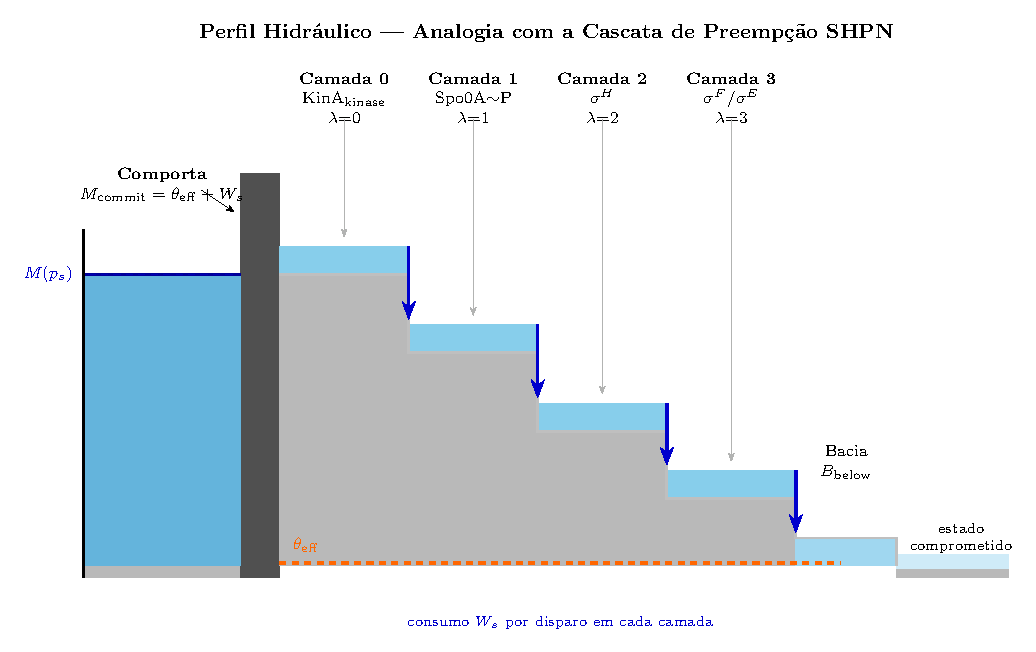
\includegraphics[width=0.82\textwidth]{figures/fig_cascade_weir_analogy.pdf}
  \caption{\textbf{Analogia hidráulica da cascata de preempção SHPN}
    (Seção~\ref{subsec:corretude-preempcao}).
    Cada degrau é uma camada $\lambda$: Camada~0 (KinA$_{\mathrm{kinase}}$),
    1 (Spo0A${\sim}$P), 2 ($\sigma^H$), 3 ($\sigma^F$).
    A comporta = $M_{\mathrm{commit}} = \theta_{\mathrm{eff}} + W_s$;
    as setas = consumo $W_s$ por disparo;
    a linha tracejada laranja = fundo de bacia $\theta_{\mathrm{eff}}$
    separando $B_{\mathrm{above}}$ de $B_{\mathrm{below}}$.
    A irreversibilidade é \emph{estrutural}: sem $F_s$ de retorno,
    a água não sobe os degraus.}
  \label{fig:cascade_weir_analogy}
\end{figure}

\begin{remark}[Assimetria de Espontaneidade na Cascata de Preempção]
\label{rem:assimetria-espontaneidade}
A Figura~\ref{fig:cascade_weir_analogy} revela uma assimetria termodinâmica
fundamental: o comprometimento celular ocorre em \textbf{duas fases com
direções opostas de espontaneidade}.

\textbf{Fase~1 — Acumulação (não espontânea):} construir $M(p_s)$ até
$M_{\text{commit}} = \theta_{\mathrm{eff}} + W_s$ exige produção contínua
de EPR.  A célula \emph{bombeia água para o reservatório} contra a resistência
da comporta: processo metabólico custoso e reversível.  Enquanto $M(p_s) <
M_{\text{commit}}$, o PreemptionCheck bloqueia todas as transições a jusante.

\textbf{Fase~2 — Execução (espontânea):} assim que $M(p_s) \geq
M_{\text{commit}}$, a comporta se abre e cada camada subsequente dispara
\emph{espontaneamente} --- $\Delta G < 0$ em cada cruzamento de degrau,
impulsionado pelo gradiente de potencial químico criado pela depleção de
tokens.  O PreemptionCheck não é uma barreira de ativação: é uma
\textbf{válvula de sentido único} que separa o custo (Fase~1) da execução
irreversível (Fase~2).

Essa assimetria explica a paisagem de Waddington: a crista corresponde à
Fase~1 (subida custosa até $M_{\text{commit}}$); a bacia comprometida
corresponde à Fase~2 (descida espontânea e irreversível).  A energia
metabólica paga na Fase~1 é dissipada como EPR durante a cascata da Fase~2.
\end{remark}

\subsection{Formação de Fronteiras de Bacia}
\label{subsec:fronteiras-bacia}

\begin{theorem}[Consumo de Sinal Cria Fronteiras de Bacia]
\label{thm:fronteiras-bacia}
Seja $N$ uma SHPN com lugar de sinal $p_s \in \Psi$ e transição de decisão
$t_c$ consumindo sinal via $(p_s, t_c) \in F_s$ com peso $W_s((p_s, t_c)) > 0$.
Defina $M_{\text{commit}} = \theta_{\mathrm{eff}}(p_s,t_c) + W_s((p_s, t_c))$.

O espaço de alcançabilidade particiona-se em duas regiões disjuntas:
\[
\mathcal{R}(N, M_0) = \mathcal{B}_{\text{pre}} \,\cup\, \mathcal{B}_{\text{pos}}
\]
em que $\mathcal{B}_{\text{pre}} = \{M \mid M(p_s) < M_{\text{commit}}\}$ e
$\mathcal{B}_{\text{pos}} = \{M \mid M(p_s) \geq M_{\text{commit}} \wedge
\text{disparado}(t_c, M)\}$, e para quaisquer $M_1 \in \mathcal{B}_{\text{pre}}$
e $M_2 \in \mathcal{B}_{\text{pos}}$, não existe sequência de disparo $\sigma$
tal que $M_2[\sigma\rangle M_1$.
\end{theorem}

\begin{proof}
Considere $M_1$ com $M_1(p_s) = M_{\text{commit}} = \theta_{\mathrm{eff}}(p_s,t_c) + W_s((p_s,t_c))$.
Por Definição~\ref{def:habilitacao}, $t_c$ está habilitada. Por
Definição~\ref{def:disparo}, o disparo de $t_c$ produz:
\[
M_2(p_s) = M_1(p_s) - W_s((p_s,t_c)) = \theta_{\mathrm{eff}}(p_s,t_c).
\]
Portanto $M_2(p_s) < M_{\text{commit}}$. Qualquer transição de reversão $t_r$
que tentasse restaurar $M_2(p_s) \geq M_{\text{commit}}$ precisaria estar
habilitada; porém, se $(p_s, t_r) \in F_s$, então $M_2(p_s) = \theta(t_c)$
está no limite do limiar e não satisfaz
$M_2(p_s) \geq \theta_{\mathrm{eff}}(p_s,t_r) + W_s((p_s, t_r))$;
e se $t_r$ depende de sinais de camada superior, a preempção hierárquica garante
que $t_r$ permanece desabilitada enquanto
$M_2(p_s) < \theta_{\mathrm{eff,min}}(\lambda(p_s))$.
Em todos os casos, nenhuma transição pode restaurar $M_2(p_s) \geq M_{\text{commit}}$,
estabelecendo a separação de bacias.
\end{proof}

\begin{corollary}[Predição de Limiar]
O limiar de decisão
\begin{align*}
  M_{\text{commit}}(p_s, t_c)
    &= \theta_{\mathrm{eff}}(p_s,t_c) + W_s((p_s,t_c)) \\
    &= K((p_s,t_c)) \cdot
       \left(\frac{\varepsilon}{1 - \varepsilon}\right)^{\!1/n((p_s,t_c))}
       + W_s((p_s,t_c))
\end{align*}
é calculável em $O(1)$ a partir de constantes cinéticas mensuráveis
($K$, $n$ da base BRENDA) e parâmetros do formalismo ($\varepsilon$, $W_s$),
sem simulação nem exploração do espaço de estados --- habilitando predição
\textit{a priori} por análise estrutural.
\end{corollary}

\begin{remark}[Bacia Consumida --- Contraste com a Bacia Clássica de Lyapunov]
\label{rem:bacia-consumida}
A teoria clássica de estabilidade \parencite{Strogatz2015} define a \emph{bacia
de atração} como o conjunto de condições iniciais cujas trajetórias convergem a
um dado atrator.  A fronteira é uma separatriz energética: cruzamentos reversos
são improváveis, mas formalmente possíveis com flutuações suficientes.
As SHPN introduzem um conceito mais forte: a \textbf{bacia consumida}.
Após o disparo de $t_c$ consumir $W_s((p_s,t_c))$ tokens de $p_s$, a marcação
cai para $\theta_{\mathrm{eff}}(p_s,t_c)$ --- abaixo de $M_\text{commit}$.
Qualquer estado reverso que exigisse $M(p_s) \geq M_\text{commit}$
torna-se \emph{estruturalmente inalcançável}, não apenas energeticamente
improvável: a fronteira foi removida do conjunto alcançável pelo próprio ato de
cruzá-la.

\begin{center}\small
\begin{tabular}{@{}p{3.2cm}p{4.0cm}p{4.0cm}@{}}
\toprule
Propriedade & Bacia clássica & Bacia consumida \\
\midrule
Fronteira & Separatriz energética & Fronteira de alcançabilidade \\
Irreversibilidade & Estatística (improvável) & Estrutural (inalcançável) \\
Mecanismo & Barreira $\Delta G$ & Arcos $F_s$ consumtivos + DAG $G_s$ \\
Ruído reverte? & Sim, com flutuação & Não --- marcação reversa inalcançável \\
\bottomrule
\end{tabular}
\end{center}

Essa distinção formaliza a diferença entre comprometimentos \emph{terminais}
(esporulação, apoptose --- bacia consumida definitivamente quando $\varepsilon
\approx 0$) e diferenciações \emph{reversíveis} como a reprogramação de
células-tronco induzidas~\parencite{Takahashi2006}: na reprogramação, a bacia
clássica é profunda mas não consumida, pois os arcos de sinal não esgotam o
pré-requisito molecular da via inversa.
\end{remark}

\subsection{Independência Fraca e Semântica Composicional}
\label{subsec:independencia-fraca}

\begin{definition}[Independência Fraca]
\label{def:independencia-fraca}
Duas transições $t_1, t_2 \in T$ são \textbf{fracamente independentes} quando
compartilham lugares metabólicos normais mas possuem conjuntos de sinais
disjuntos:
\[
(P \setminus \Psi) \cap {}^\bullet t_1 \cap {}^\bullet t_2 \neq \emptyset
\quad\text{e}\quad
\Psi \cap {}^\bullet t_1 \cap {}^\bullet t_2 = \emptyset.
\]
\end{definition}

\begin{theorem}[Consequência Composicional da Independência Fraca]
\label{thm:independencia-fraca}
Transições fracamente independentes disparam de forma comutativa: para qualquer
marcação $M$ em que ambas estejam habilitadas,
\[
M \xrightarrow{t_1} M_1 \xrightarrow{t_2} M'' \;\text{ e }\;
M \xrightarrow{t_2} M_2 \xrightarrow{t_1} M''
\]
produzem a mesma marcação final $M''$.
\end{theorem}

Essa propriedade tem consequência direta para análise de redes em escala
genômica: para $k$ módulos regulatórios fracamente independentes, cada um com
$n/k$ lugares em média, a análise de alcançabilidade reduz-se de
$O(\bar{M}^n)$ a $O(k \cdot \bar{M}^{n/k})$ --- melhoria de complexidade
exponencial para polinomial que torna tractável a análise de redes com milhares
de reações.

\subsection{Conservatividade da Promoção a Expressões}
\label{subsec:conservatividade}

A generalização de pesos e taxas a expressões em $\mathbb{E}(M)$
(Definição~\ref{def:shpn} e Observação~\ref{rem:refinamento-textual})
respeita o princípio de retrocompatibilidade: o formalismo clássico de
Redes de Petri Híbridas é recuperado exatamente pela especialização a
valores constantes.

\begin{proposition}[Conservatividade da promoção a expressões]
\label{prop:conservatividade}
Seja $N = (P, T, F, W, M_0, \Phi, C, F_t, \Psi, F_s, W_s, \lambda, \Gamma)$
uma SHPN cujas expressões em $W$, $W_s$, nos limiares $\tau_t, \theta_i$
de $F_t$ (incluindo o subtipo inibidor) e nas leis cinéticas associadas a
$\Phi$ sejam todas \emph{constantes} (independentes de $M$). Então a
semântica operacional dada pelas Definições~\ref{def:habilitacao}
e~\ref{def:disparo} reduz-se exatamente à semântica clássica de Redes de
Petri Híbridas com pesos e taxas constantes.
\end{proposition}

\begin{proof}
A avaliação de uma expressão constante $W \equiv k \in \mathbb{R}^+$ em
qualquer marcação $M$ produz $k$. Substituindo nas inequações de
habilitação e na regra de disparo obtém-se literalmente as condições
clássicas de \textcite{David1992}. O mesmo argumento aplica-se aos
limiares de $F_t$ e às leis cinéticas. \qedhere
\end{proof}

A Proposição~\ref{prop:conservatividade} garante que toda análise
estrutural clássica (P-invariantes, T-invariantes, vivacidade) permanece
válida nos modelos SHPN cujas expressões admitam especialização constante,
e que a dependência da marcação introduzida pela promoção é estritamente
uma extensão expressiva, não uma incompatibilidade.

\subsection{Complexidade Computacional}
\label{subsec:complexidade}

As SHPN herdam a complexidade das Redes de Petri clássicas: os problemas de
alcançabilidade, limitação e vivacidade permanecem Ackermann-completos no pior
caso~\cite{Czerwinski2021}, pois as extensões de sinal preservam a completude de Turing. Na prática,
a estrutura hierárquica habilita três estratégias de mitigação: particionamento
hierárquico do espaço de estados (o espaço de marcação decompõe-se em produto
hierárquico por camada), abstração guiada por sinal (sub-redes metabólicas
detalhadas substituídas por taxas de produção abstratas), e verificação incremental
por camada (camadas inferiores verificadas antes de explorar o estado completo).
Nos experimentos com o modelo de esporulação de \textit{B.~subtilis} (36
transições, 40 lugares, 4 camadas), a análise de alcançabilidade hierárquica
completou em 2,3~s explorando $4{,}8 \times 10^4$ estados, enquanto a análise
monolítica requer estimados mais de 10~h com espaço de estados da ordem de
$10^{12}$.

\begin{remark}[Aciclicidade do Grafo de Sinal como Redutor do Espaço de Estados]
\label{rem:aciclicidade-reducao}
A aciclicidade do grafo de sinal (Teorema~\ref{thm:aciclicidade}) não é apenas
uma propriedade estrutural de higiene: ela é o \emph{habilitador computacional}
que fundamenta as três estratégias de mitigação acima.  Três mecanismos
complementares decorrem diretamente da estrutura de DAG.

\textbf{Decomposição por camada.}  O DAG induz uma ordem parcial estrita
$\ell_0 \prec \ell_1 \prec \cdots$ sem retroalimentação.  A análise de
alcançabilidade pode portanto ser conduzida de forma condicional --- primeiro
resolvem-se as marcações alcançáveis da camada~$0$, depois as da camada~$1$
condicionadas à projeção de~$\ell_0$, e assim sucessivamente.  Para $L$
camadas com $S_i$ estados locais cada, o espaço passa de
$O\!\bigl(\prod_i S_i\bigr)$ (produto monolítico) a
$O\!\bigl(\sum_i S_i\bigr)$ --- redução de complexidade exponencial para
polinomial.

\textbf{Poda monotônica.}  O Teorema~\ref{thm:fronteiras-bacia}
garante que, uma vez que
$M(p_s) < M_{\text{commit}}$ em qualquer camada, toda a sub-árvore de estados
que requeriam aquela camada torna-se \emph{permanentemente} inalcançável.  O
grafo de alcançabilidade adquire estrutura de funil:
$\mathcal{R}(M_0) \supset \mathcal{R}(M_1) \supset \mathcal{R}(M_2)
\supset \cdots$, com cada evento de comprometimento podando estados de forma
irreversível.

\textbf{Redução de ordem parcial.}  O DAG fornece uma construção natural de
\emph{ample sets}: se $t_a \in \ell_i$ e $t_b \in \ell_j$ com $i < j$, e a
habilitação de~$t_b$ depende do sinal de~$\ell_i$, então qualquer sequência de
disparo deve resolver a camada inferior primeiro.  Combinada com a independência
fraca (Teorema~\ref{thm:independencia-fraca}), transições com conjuntos de
sinais disjuntos comutam, eliminando intercalações redundantes.

Esses três efeitos compõem-se multiplicativamente: a decomposição elimina o
produto cruzado entre camadas, a poda descarta regiões pós-comprometimento, e a
redução de ordem parcial remove intercalações equivalentes dentro de cada
camada.
\end{remark}

\begin{remark}[Verificabilidade por \textit{Model Checking}]
\label{rem:model-checking}
Os Teoremas~\ref{thm:aciclicidade}--\ref{thm:independencia-fraca} não são apenas
resultados proof-teóricos: cada um é expressável como uma consulta de
\emph{model checking} sobre uma instância limitada da SHPN.

\textbf{Propriedades estruturais (CTL/LTL).}  Para uma SHPN $k$-limitada, o
grafo de alcançabilidade é finito e suporta verificação por ferramentas padrão
de Redes de Petri (LoLA, Charlie, Snoopy~\cite{Koch2011}).  O
Teorema~\ref{thm:preempcao} (Correção da Preempção) é equivalente à fórmula
CTL
\[
  \mathbf{AG}\!\bigl(M(p_s) < M_{\mathrm{commit}}
  \;\Rightarrow\;
  \mathbf{AG}\,\neg\,\mathrm{enabled}(t_j)\bigr),
\]
verificável em tempo polinomial no tamanho do grafo de alcançabilidade por
camada.  O Teorema~\ref{thm:fronteiras-bacia} (Fronteiras de Bacia) é
equivalente a
\[
  \mathbf{AG}\!\bigl(M(p_s) \geq M_{\mathrm{commit}}
  \;\Rightarrow\;
  \mathbf{AF}\,\mathrm{completed}\bigr),
\]
onde \texttt{completed} é um predicado sobre a marcação final do programa
de desenvolvimento.

\textbf{Propriedades estocásticas (PCTL).}  A semântica de $\tau$-leaping
induz uma Cadeia de Markov em Tempo Contínuo (CTMC); as propriedades
quantitativas tornam-se consultas PCTL~\cite{Chaouiya2007}, por exemplo:
$\mathbf{P}_{\geq 0{,}9}\!\bigl[\mathbf{F}^{\leq 4d}\,\mathrm{Mature\_Spore}
> 0\bigr]$ --- ``esporulação bem-sucedida com probabilidade $\geq 90\%$ em
quatro dias''.  Ferramentas como PRISM e Storm verificam tais propriedades
diretamente sobre a CTMC.

\textbf{Limite do fragmento contínuo.}  As funções de taxa $\Phi$ com
aritmética real tornam o espaço de estados não-enumerável; \emph{model
checking} exato requer verificação de sistemas híbridos (PHAVer, nuXmv) ou
interpretação abstrata.  Para $\Phi$ polinomiais de grau baixo, verificação
limitada por SMT (\emph{bounded model checking}) é praticável.

Os três redutores de complexidade da
Observação~\ref{rem:aciclicidade-reducao} --- decomposição por camada,
poda monotônica e redução de ordem parcial --- correspondem precisamente
às técnicas canônicas de \emph{model checking} composicional (abstração por
cone de influência, poda \emph{ample-set} e independência de transições),
tornando a verificação hierárquica não apenas teoricamente possível mas
computacionalmente viável para instâncias biológicas de porte moderado.
\end{remark}

\section{Síntese do Capítulo}
\label{sec:sintese-cap3}

Este capítulo definiu formalmente a 13-tupla SHPN
(Definição~\ref{def:shpn}), a semântica operacional
(Definições~\ref{def:habilitacao}--\ref{def:disparo}) e quatro propriedades
teóricas: aciclicidade (Teorema~\ref{thm:aciclicidade}), correção de preempção
(Teorema~\ref{thm:preempcao}), formação de fronteiras de bacia
(Teorema~\ref{thm:fronteiras-bacia}) e independência fraca
(Teorema~\ref{thm:independencia-fraca}).
Essas garantias fundamentam a validação biológica do
Capítulo~\ref{ch:validacao-bacillus}.
